\chapter{Kapitel}

\section{Unterkapitel}

\subsection{Unterunterkapitel}

\lipsum[2]

\begin{figure}[h!]
	\centering
		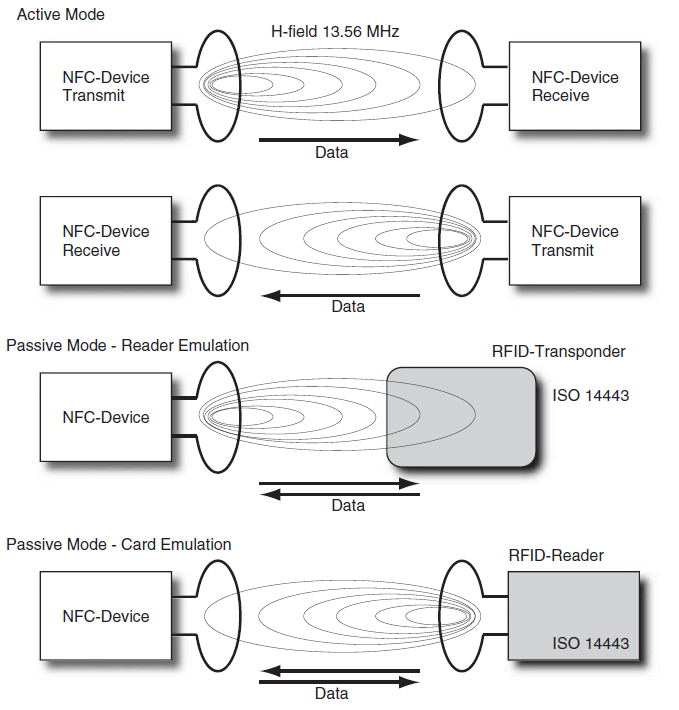
\includegraphics[width=0.6\textwidth]{images/nfc_communication}
		\vspace*{0pt}
	\caption[NFC operating modes]{NFC operating modes \citep[p.~58]{Finkenzeller.2010}}
	\label{fig:nfc_communication}
\end{figure}

\lipsum[2]

\begin{equation}
	\overline{x} = \frac 1n \sum^n_{i=1} x_i
\end{equation}

\lipsum[2] 

My reference to Tabelle~\ref{tbl:beispieltabelle1}.

% Zur Generierung von Tabellen kann das Excel-Plugin "Excel2Latex" verwendet werden
\begin{table}
	\centering
	
		\begin{tabular}{|l|l|r|}
		\hline
			\textbf{Farbe} & \textbf{Form} & \textbf{Zahl} \\
		\hline
			Rot & Rechteck & 100 \\
		\hline
			Blau & Kreis & 99 \\
		\hline
			Gelb & Dreieck & 98 \\
		\hline
		\end{tabular}
		\caption{Another table layout}
	    \label{tbl:beispieltabelle1}
	
\end{table}

\subsection{Unterunterkapitel 2}

\section{Unterkapitel 2}

\section{Unterkapitel 3}